\documentclass[a4paper,12pt]{article}
\usepackage[utf8]{inputenc}
\usepackage[T1]{fontenc}
\usepackage{babel}
\selectlanguage{ngerman}
\usepackage{amsmath}
\usepackage{amssymb}
\usepackage{amsthm}
\usepackage{geometry}
\usepackage{graphicx}
\usepackage[hidelinks]{hyperref}
\usepackage{listings}
\usepackage{xcolor}
\usepackage{enumitem}
\usepackage[activate={true,nocompatibility},final,tracking=true,kerning=true,
            spacing=true,factor=1100,stretch=15,shrink=15]{microtype}
\usepackage{booktabs}
\usepackage{array}
\usepackage{caption}
\usepackage{xurl}

% Zeilenumbrüche verbessern – verhindert Überlauf über den rechten Rand
\setlength{\emergencystretch}{3em}
\setlength{\hfuzz}{1pt}

\geometry{margin=2.5cm}

\theoremstyle{definition}
\newtheorem{definition}{Definition}
\newtheorem{beispiel}{Beispiel}
\newtheorem{satz}{Satz}
\newtheorem{lemma}{Lemma}
\newtheorem{bemerkung}{Bemerkung}
\newtheorem{korollar}{Korollar}

\setlist[itemize,1]{label=--}

% ---------- Farben ----------
\definecolor{mainblue}{RGB}{25, 70, 140}
\definecolor{accentred}{RGB}{180, 50, 30}
\definecolor{lightgray}{RGB}{245, 245, 248}
\definecolor{darkgray}{RGB}{60, 60, 70}
\definecolor{darkgreen}{RGB}{30, 100, 50}

\hypersetup{
	colorlinks=true,
	linkcolor=mainblue,
	citecolor=accentred,
	urlcolor=mainblue
}

\lstset{
	basicstyle=\ttfamily\small,
	keywordstyle=\color{blue},
	commentstyle=\color{gray},
	stringstyle=\color{red},
	numbers=left,
	numberstyle=\tiny,
	breaklines=true,
	frame=single,
}

\title{\textbf{Laser-basierte Orthogonalitätskontrolle\\für Bohrmaschinen}\\[0.5em]
\large Formale Modellierung, Messtechnik und Systemarchitektur\\
eines optischen Winkelsensors}
\author{Stephan Epp}
\date{18. Juni 2026}

\begin{document}

\maketitle

\begin{abstract}
Die exakte Orthogonalität eines Bohrers zur Werkstückoberfläche ist in der Präzisionsfertigung,
im Handwerk und in der Medizintechnik von entscheidender Bedeutung. Selbst geringe Winkelabweichungen
führen zu Maßfehlern, erhöhtem Werkzeugverschleiß und struktureller Schwächung des Bauteils.
Die vorliegende Arbeit stellt ein neuartiges Sensorsystem vor, das mittels eines monochromatischen
Laserstrahls und eines zweidimensionalen Positionssensors (2D-PSD oder CMOS-Array) kontinuierlich
und in Echtzeit prüft, ob der Bohrer orthogonal zur Bohrfläche ausgerichtet ist.
Das System projiziert den Laserstrahl koaxial zur Bohrachse auf die Werkstückoberfläche oder --
bei Durchbohrungen -- auf eine hinter dem Werkstück angebrachte Referenzfläche und wertet die
Ablenkung des Lichtflecks geometrisch aus.
Wir leiten das vollständige mathematische Modell formal her, beweisen die Korrektheit
der Winkelberechnung sowie die Eindeutigkeit der Messung, analysieren Messunschärfen
und Fehlerquellen und beschreiben die Systemarchitektur und Echtzeitalgorithmik.
Abschließend wird ein umfangreicher Ausblick auf Erweiterungen und Anwendungsfelder gegeben.
\end{abstract}

\tableofcontents
\newpage

% ═══════════════════════════════════════════════════════════════════════════════
\section{Einführung}

Bohrmaschinen aller Art -- von handgeführten Akkubohrern über Tischbohrmaschinen bis hin zu
Industrie-CNC-Bearbeitungszentren -- leiden bei manueller Führung unter dem Problem der
Winkelabweichung: Der Bohrer weicht von der idealen Senkrechtachse zur Werkstückoberfläche ab,
was zu ovalen Bohrlochdurchmessern, Schrägsitzen von Verbindungselementen und Rissen im Material
führen kann~\cite{klocke2018fertigungsverfahren, toennis2020messtechnik}.

\subsection{Problemstellung}

Gegeben sei eine Bohrmaschine mit Bohrerachse~$\mathbf{a} \in \mathbb{R}^3$, $\|\mathbf{a}\|=1$,
und eine Werkstückoberfläche, die durch ihren Normalenvektor $\mathbf{n} \in \mathbb{R}^3$,
$\|\mathbf{n}\|=1$, charakterisiert wird.
Das \textbf{Orthogonalitätsproblem} lautet:

\begin{itemize}
  \item Berechne den Winkel $\alpha = \angle(\mathbf{a}, \mathbf{n}) \in [0^\circ, 90^\circ]$
    zwischen Bohrerachse und Oberflächennormale.
  \item Zeige in Echtzeit an, ob $\alpha \leq \alpha_{\mathrm{tol}}$ gilt
    (orthogonale Bohrung) oder $\alpha > \alpha_{\mathrm{tol}}$
    (Winkelabweichung außerhalb der Toleranz).
  \item Quantifiziere die Richtung und das Ausmaß der Abweichung, damit der
    Bediener oder eine CNC-Achse korrigieren kann.
\end{itemize}

\subsection{Lösungsansatz}

Die vorliegende Arbeit löst dieses Problem durch ein optisches Messverfahren:
Ein kollimierter Laserstrahl wird koaxial zur Bohrerachse ausgesendet.
Bei orthogonaler Ausrichtung ($\alpha=0$) trifft der Strahl das Bohrziel oder
eine Referenzebene im Zentrum eines kalibrierten 2D-Detektors.
Jede Winkelabweichung $\alpha>0$ bewirkt eine proportionale Lateralverschiebung
$\delta$ des Laserspots, die von einem Positionsdetektor (2D-PSD oder CMOS-Kamera)
erfasst und in einen Winkel umgerechnet wird.

\begin{figure}[h]
  \centering
  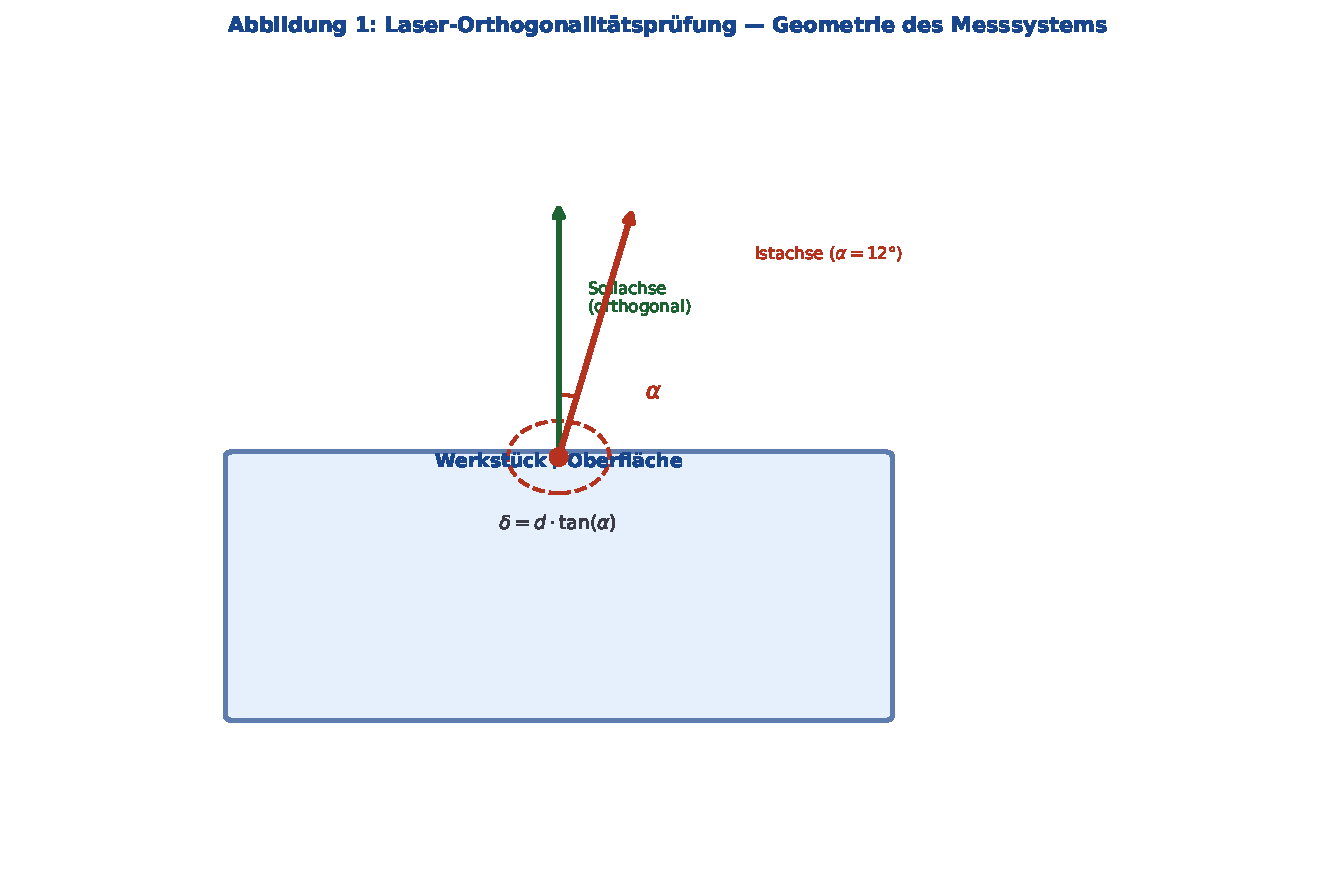
\includegraphics[width=0.75\textwidth]{plot1_geometrie.png}
  \caption{Geometrie des Laser-Orthogonalitätssensors: Der grüne Vektor
    bezeichnet die Sollachse (orthogonal zur Oberfläche), der rote Vektor
    die Istachse mit Winkelabweichung~$\alpha$. Die Lateralablenkung
    $\delta = d \cdot \tan\alpha$ am Detektor ist das Messsignal.}
  \label{fig:geometrie}
\end{figure}

\subsection{Überblick über den Stand der Technik}

Bestehende Lösungen für die Orthogonalitätskontrolle umfassen:
\begin{itemize}
  \item \textbf{Mechanische Anschläge:} Bohrständer und Führungshilfen, die
    jedoch keine Rückmeldung liefern und bei nicht-planaren Oberflächen versagen.
  \item \textbf{Wasserwaagen und digitale Neigungssensoren:} MEMS-Beschleunigungs\-messer,
    die jedoch ausschließlich die absolute Ausrichtung zur Schwerkraft messen --
    für geneigt liegende Werkstücke ungeeignet~\cite{fraden2010handbook}.
  \item \textbf{Kamerasysteme:} Hochpräzise, aber teuer und empfindlich gegenüber
    Spänen und Kühlmittel~\cite{jaehne2005digitale}.
  \item \textbf{Laserbasierte Systeme:} Existierende industrielle Lösungen sind
    als separate stationäre Messgeräte konzipiert, nicht als in die Ma\-schine
    integrierte Echtzeit\-sensoren~\cite{schwenke2008geometric}.
\end{itemize}

Das hier vorgestellte System schließt diese Lücke durch eine kompakte,
in den Bohrerhalter integrierbare Sensorik mit digitalem Echtzeitfeedback.

% ═══════════════════════════════════════════════════════════════════════════════
\section{Mathematisches Grundlagenmodell}

\subsection{Koordinatensystem und Definitionen}

\begin{definition}[Bohrerachse und Oberflächennormale]
  Sei $\mathcal{K}$ ein kartesisches Koordinatensystem mit Ursprung~$O$ im
  Schnittpunkt der Bohrerachse mit der Werkstückoberfläche.
  Die \emph{Bohrerachse} ist der Einheitsvektor
  \[
    \mathbf{a} = (a_x, a_y, a_z)^\top \in \mathbb{R}^3, \quad \|\mathbf{a}\|_2 = 1.
  \]
  Die \emph{Oberflächennormale} am Auftreffpunkt ist der Einheitsvektor
  \[
    \mathbf{n} = (n_x, n_y, n_z)^\top \in \mathbb{R}^3, \quad \|\mathbf{n}\|_2 = 1.
  \]
\end{definition}

\begin{definition}[Orthogonalitätswinkel]
  Der \emph{Orthogonalitätswinkel} $\alpha \in [0^\circ, 90^\circ]$ zwischen Bohrerachse
  und Oberflächennormale ist definiert als:
  \[
    \alpha = \arccos\!\bigl(\mathbf{a} \cdot \mathbf{n}\bigr)
           = \arccos\!\bigl(|\mathbf{a}^\top \mathbf{n}|\bigr).
  \]
  Gilt $\alpha = 0^\circ$, so ist die Bohrung orthogonal zur Oberfläche.
\end{definition}

\begin{definition}[Laserstrahl]
  Der Laserstrahl sei als Halbgerade
  \[
    \ell(t) = P_0 + t\,\hat{\mathbf{d}}, \quad t \geq 0,
  \]
  modelliert, wobei $P_0 \in \mathbb{R}^3$ die Ausgabeapertur des Lasers
  und $\hat{\mathbf{d}} = \mathbf{a}$ (koaxial zur Bohrerachse)
  der Richtungsvektor des Strahls ist.
\end{definition}

\begin{definition}[Referenzebene und Detektor]
  Die \emph{Referenzebene}~$\Pi$ ist in einem Abstand~$d > 0$ hinter dem
  Werkstück (oder an der Bohrspitze) senkrecht zur Sollachse angebracht:
  \[
    \Pi = \bigl\{P \in \mathbb{R}^3 \;\big|\; \mathbf{n}_0^\top P = d\bigr\},
  \]
  wobei $\mathbf{n}_0 = (0,0,1)^\top$ die Sollrichtung bezeichnet.
  Der 2D-Positionsdetektor ist in $\Pi$ zentriert auf~$O' = d \cdot \mathbf{n}_0$.
\end{definition}

\subsection{Geometrisches Modell der Ablenkung}

\begin{satz}[Lateralablenkung]
  \label{satz:ablenkung}
  Weicht die Bohrerachse $\mathbf{a}$ um den Winkel~$\alpha$ von der
  Sollachse~$\mathbf{n}_0$ ab, so verschiebt sich der Laserspot auf der
  Referenzebene~$\Pi$ (Abstand~$d$) lateral um:
  \[
    \delta = d \cdot \tan\alpha.
  \]
\end{satz}

\begin{proof}
  Sei ohne Einschränkung das Koordinatensystem so gewählt, dass
  $\mathbf{n}_0 = (0,0,1)^\top$ und die Abweichungsebene die $xz$-Ebene ist.
  Der tatsächliche Laserrichtungsvektor lautet dann:
  \[
    \hat{\mathbf{d}} = (\sin\alpha,\; 0,\; \cos\alpha)^\top.
  \]
  Der Strahl $\ell(t) = t\,\hat{\mathbf{d}}$ schneidet die Ebene
  $\{z = d\}$ bei:
  \[
    t^* = \frac{d}{\cos\alpha}.
  \]
  Die $x$-Koordinate des Auftreffpunkts beträgt:
  \[
    x^* = t^* \sin\alpha = \frac{d \sin\alpha}{\cos\alpha} = d \tan\alpha. \qedhere
  \]
\end{proof}

\begin{korollar}[Winkelrekonstruktion]
  \label{kor:winkel}
  Aus der gemessenen Lateralverschiebung $\hat{\delta}$ des Laserspots
  und dem bekannten Abstand~$d$ ergibt sich der Orthogonalitätswinkel:
  \[
    \hat{\alpha} = \arctan\!\left(\frac{\hat{\delta}}{d}\right).
  \]
\end{korollar}

\begin{proof}
  Direkte Umkehrung von Satz~\ref{satz:ablenkung}:
  $\delta = d\tan\alpha \Leftrightarrow \alpha = \arctan(\delta/d)$. \qedhere
\end{proof}

\begin{figure}[h]
  \centering
  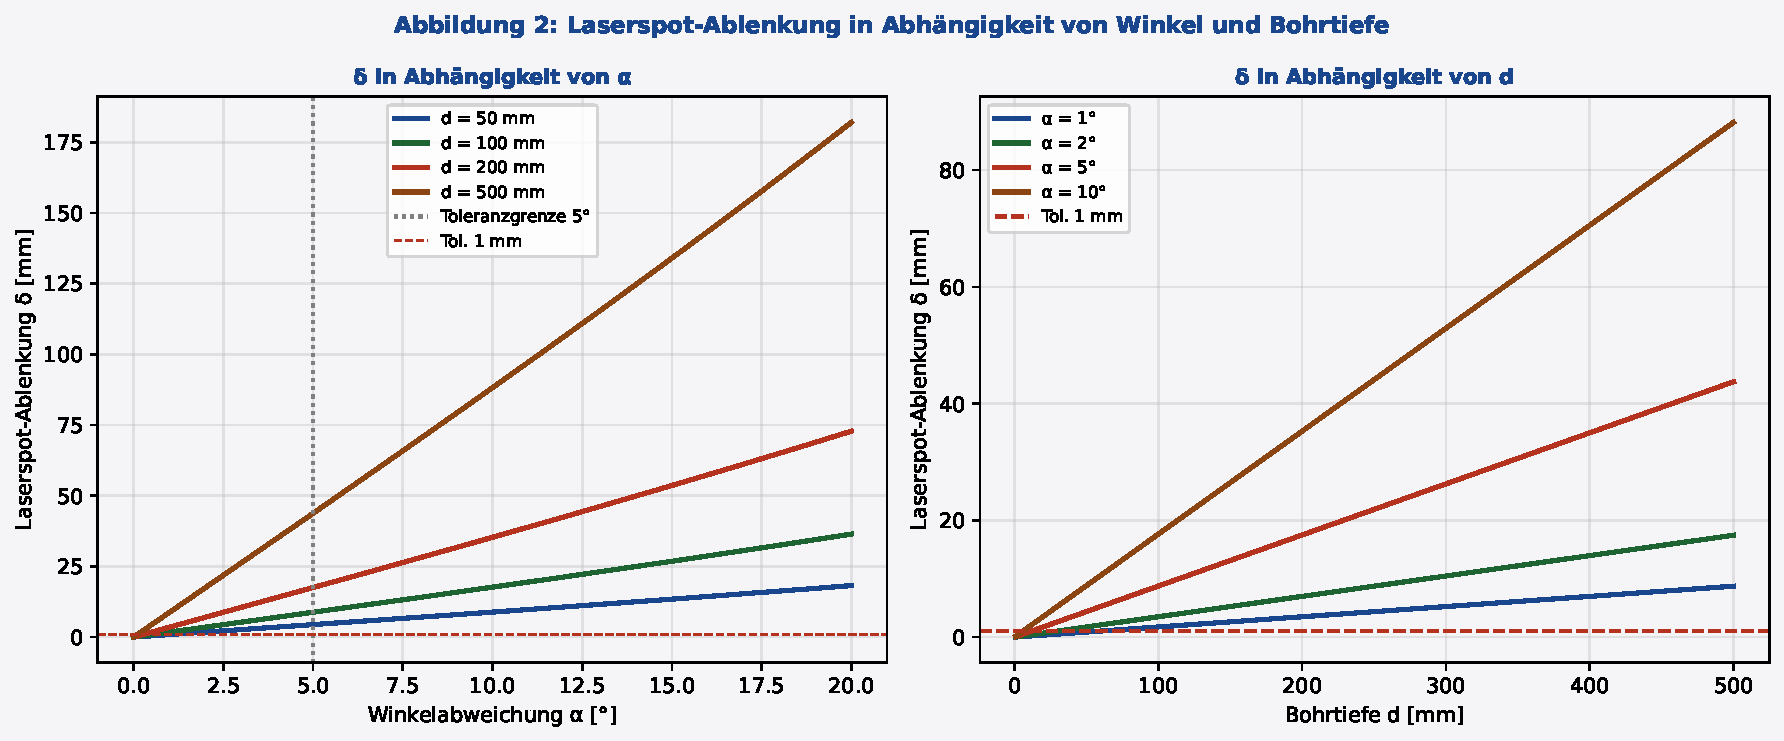
\includegraphics[width=\textwidth]{plot2_ablenkung.png}
  \caption{Laserspot-Ablenkung $\delta$ als Funktion des Winkels~$\alpha$
    (links) und der Bohrtiefe/Detektorabstand~$d$ (rechts) für
    verschiedene Parameterkombinationen. Die rote gestrichelte Linie
    markiert die typische Toleranzgrenze von 1\,mm Ablenkung; die graue
    Punktlinie links kennzeichnet eine Winkeltoleranz von 5°.}
  \label{fig:ablenkung}
\end{figure}

\subsection{Zweidimensionale Richtungsbestimmung}

Im allgemeinen dreidimensionalen Fall zeigt die Ablenkung nicht nur Betrag,
sondern auch Richtung an. Der Laserspot trifft den Detektor im Punkt
$(x^*, y^*)^\top \in \mathbb{R}^2$.

\begin{satz}[2D-Winkelrekonstruktion]
  \label{satz:2d}
  Sei der gemessene Spotmittelpunkt auf dem Detektor
  $\hat{\mathbf{p}} = (\hat{x}, \hat{y})^\top$.
  Dann gilt:
  \begin{align}
    \hat{\delta}   &= \|\hat{\mathbf{p}}\|_2 = \sqrt{\hat{x}^2 + \hat{y}^2}, \\
    \hat{\alpha}   &= \arctan\!\left(\frac{\hat{\delta}}{d}\right), \\
    \hat{\varphi}  &= \operatorname{atan2}(\hat{y}, \hat{x}),
  \end{align}
  wobei $\hat{\alpha}$ der Tiltwinkel und $\hat{\varphi} \in [0^\circ, 360^\circ)$ die
  Richtung der Abweichung (Azimut) in der Detektorebene bezeichnet.
\end{satz}

\begin{proof}
  Da der Laserstrahl $\hat{\mathbf{d}} = (\sin\alpha_x, \sin\alpha_y, \sqrt{1-\sin^2\alpha_x-\sin^2\alpha_y})^\top$ für kleine Winkel die Linearisierung
  $\hat{\mathbf{d}} \approx (\alpha_x, \alpha_y, 1-\tfrac{1}{2}(\alpha_x^2+\alpha_y^2))^\top$
  erlaubt, ergibt sich der Auftreffpunkt auf $\{z=d\}$ zu
  $x^* \approx d\alpha_x$, $y^* \approx d\alpha_y$.
  Für beliebige Winkel liefert Satz~\ref{satz:ablenkung} komponentenweise
  $x^* = d\tan\alpha_x$, $y^* = d\tan\alpha_y$.
  Der Gesamtbetrag ergibt sich zu $\delta = \sqrt{(x^*)^2+(y^*)^2}$,
  woraus Korollar~\ref{kor:winkel} komponentenweise anwendbar ist. \qedhere
\end{proof}

% ═══════════════════════════════════════════════════════════════════════════════
\section{Sensortechnologie}

\subsection{Laserquellen}

Als Lichtquelle eignen sich kollimierte Halbleiterlaserdioden im sichtbaren
Spektrum (600--680\,nm, rot) mit einer Ausgangsleistung von $P \leq 1\,\mathrm{mW}$
(Laserklasse~1 oder~2 nach IEC~60825-1~\cite{iec60825}).
Der Strahl wird durch eine Sammellinse ($f = 20$--$50\,\mathrm{mm}$) auf einen
Fokusdurchmesser von $d_0 \leq 0{,}5\,\mathrm{mm}$ kollimiert.

\begin{definition}[Divergenz des Laserstrahls]
  Die Divergenz $\theta_{\mathrm{div}}$ eines Gaußstrahls mit Taillenradius $w_0$
  und Wellenlänge $\lambda$ ist:
  \[
    \theta_{\mathrm{div}} = \frac{\lambda}{\pi w_0}.
  \]
  Für $\lambda = 650\,\mathrm{nm}$, $w_0 = 0{,}25\,\mathrm{mm}$ ergibt sich
  $\theta_{\mathrm{div}} \approx 0{,}83\,\mathrm{mrad}$, was einer Spotaufweitung
  von $\Delta r \approx 0{,}83\,\mu\mathrm{m}$ pro Millimeter Propagationsweg entspricht.
\end{definition}

\subsection{Positionsdetektoren}

\subsubsection{2D-PSD (Position Sensitive Detector)}

Ein 2D-PSD besteht aus einem pin-Photodioden-Substrat mit vier Elektroden.
Der Fotostrom teilt sich proportional zum Abstand des Lichtflecks von den
Elektroden auf:
\[
  \hat{x} = \frac{(I_1 + I_2) - (I_3 + I_4)}{I_1 + I_2 + I_3 + I_4} \cdot \frac{L}{2},
  \qquad
  \hat{y} = \frac{(I_1 + I_4) - (I_2 + I_3)}{I_1 + I_2 + I_3 + I_4} \cdot \frac{L}{2},
\]
wobei $I_k$ die Photoströme an den vier Ecken und $L$ die Kantenlänge des Sensors
ist~\cite{walraven1985position}.

\begin{lemma}[Linearität des PSD]
  Die Positionsbestimmung mittels 2D-PSD ist linear in der Spotposition,
  sofern der gesamte Strahl auf der aktiven Fläche verbleibt.
\end{lemma}

\begin{proof}
  Die Proportionalität des Photostroms zur Bestrahlungsstärke und die
  Kirchhoff'schen Gesetze im Widerstandsnetzwerk des Substrats implizieren eine
  lineare Strom-Positions-Kennlinie, sofern der Spot vollständig auf dem Substrat
  liegt und die Randeffekte vernachlässigt werden können~\cite{walraven1985position}.
  \qedhere
\end{proof}

\subsubsection{CMOS-Bildarray als Alternative}

Bei Einsatz eines CMOS-Sensors der Auflösung $M \times N$ Pixel mit Pixelgröße $p$
[in mm] ergibt sich der Spotmittelpunkt durch den gewichteten Schwerpunkt der
Intensitätsverteilung:
\[
  \hat{x} = \frac{\sum_{i,j} x_{ij} \cdot I_{ij}}{\sum_{i,j} I_{ij}},
  \qquad
  \hat{y} = \frac{\sum_{i,j} y_{ij} \cdot I_{ij}}{\sum_{i,j} I_{ij}}.
\]
Die theoretische Positionsauflösung beträgt:
\[
  \sigma_{\mathrm{pos}} = \frac{p}{\sqrt{N_{\mathrm{ph}}}},
\]
wobei $N_{\mathrm{ph}}$ die Anzahl der detektierten Photonen ist.

\begin{figure}[h]
  \centering
  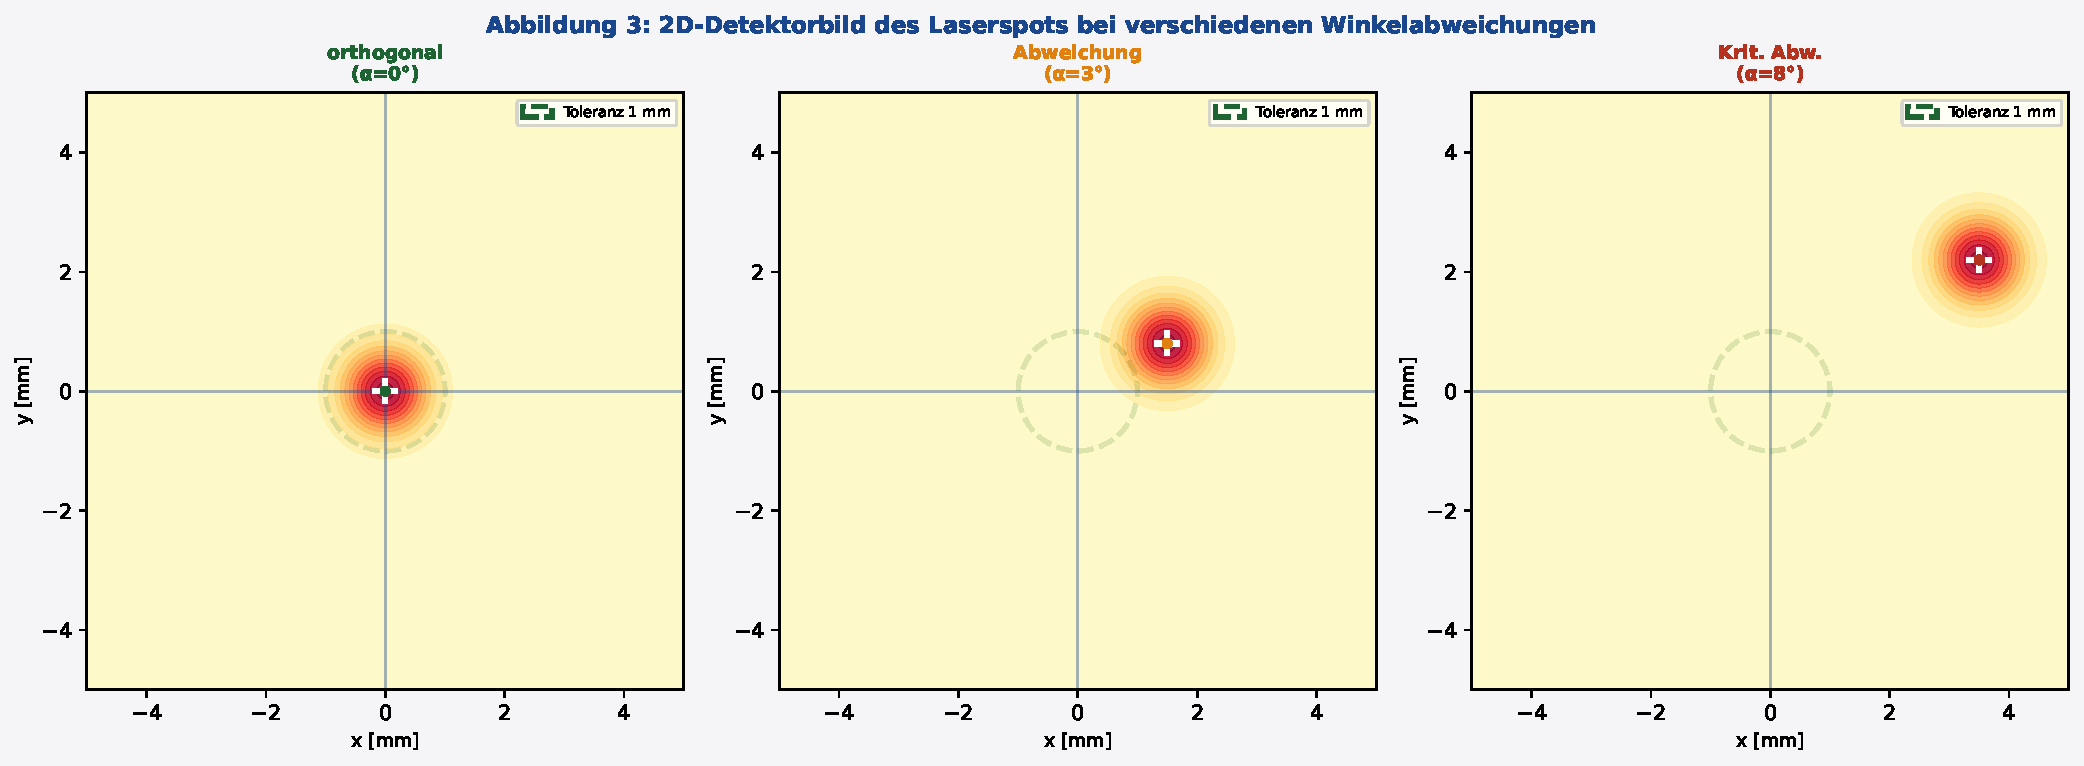
\includegraphics[width=\textwidth]{plot3_heatmap.png}
  \caption{2D-Detektorbild (simuliertes CMOS-Array) des Gaußförmigen Laserspots
    bei drei Winkelabweichungen. Links: orthogonale Bohrung ($\alpha=0^\circ$), Spot
    im Zentrum; Mitte: leichte Abweichung ($\alpha=3^\circ$, $\delta\approx1{,}5\,\mathrm{mm}$
    bei $d=30\,\mathrm{mm}$); rechts: kritische Abweichung ($\alpha=8^\circ$, außerhalb
    der grünen Toleranzzone). Die grüne Kreislinie markiert die Toleranzgrenze
    von 1\,mm.}
  \label{fig:heatmap}
\end{figure}

% ═══════════════════════════════════════════════════════════════════════════════
\section{Formale Korrektheit und Eindeutigkeitsnachweise}

\subsection{Eindeutigkeit der Winkelrekonstruktion}

\begin{satz}[Eindeutigkeit]
  \label{satz:eindeutigkeit}
  Die Abbildung $\Phi: \alpha \mapsto \delta = d\tan\alpha$ ist für
  $\alpha \in [0^\circ, 90^\circ)$ und festes $d > 0$ streng monoton wachsend und damit
  injektiv. Insbesondere entspricht jedem gemessenen $\delta \geq 0$ genau ein
  $\alpha \in [0^\circ, 90^\circ)$.
\end{satz}

\begin{proof}
  Die Funktion $\tan: [0^\circ, 90^\circ) \to [0, +\infty)$ ist streng monoton wachsend,
  da $\frac{d}{d\alpha}\tan\alpha = \frac{1}{\cos^2\alpha} > 0$ für alle
  $\alpha \in [0^\circ, 90^\circ)$. Multiplikation mit dem festen Faktor $d > 0$ bewahrt
  die strenge Monotonie. Nach dem Satz von der Umkehrfunktion existiert daher
  die eindeutige Umkehrabbildung $\alpha = \arctan(\delta/d)$. \qedhere
\end{proof}

\subsection{Robustheit gegenüber Rauschen}

Sei $\tilde{\delta} = \delta + \varepsilon$ die verrauschte Messung mit
additivem Rauschen $\varepsilon \sim \mathcal{N}(0, \sigma^2)$.

\begin{lemma}[Fehlerfortpflanzung]
  \label{lem:fehler}
  Der Fehler in der Winkelschätzung aufgrund des Messrauschens $\varepsilon$
  beträgt in erster Ordnung:
  \[
    \Delta\hat{\alpha} \approx \frac{\sigma}{d(1 + (\delta/d)^2)}
    = \frac{\sigma}{d\cos^{-2}\hat{\alpha}}
    = \frac{\sigma \cos^2\hat{\alpha}}{d}.
  \]
\end{lemma}

\begin{proof}
  Sei $f(\delta) = \arctan(\delta/d)$.
  Die lineare Fehlerfortpflanzung liefert:
  \[
    \sigma_{\hat{\alpha}} = |f'(\delta)| \cdot \sigma
    = \frac{1/d}{1+(\delta/d)^2} \cdot \sigma
    = \frac{\sigma/d}{1+\tan^2\hat{\alpha}}
    = \frac{\sigma \cos^2\hat{\alpha}}{d}. \qedhere
  \]
\end{proof}

\begin{korollar}[Optimale Messauflösung bei kleinen Winkeln]
  Bei orthogonaler Ausrichtung ($\hat{\alpha} \approx 0$) ist die Winkel\-auflösung maximal:
  \[
    \sigma_{\hat{\alpha}} \approx \frac{\sigma}{d}.
  \]
  Für einen Detektorabstand $d = 100\,\mathrm{mm}$ und eine Positionsauflösung
  $\sigma = 0{,}05\,\mathrm{mm}$ ergibt sich eine Winkelauflösung von
  $\sigma_{\hat{\alpha}} \approx 0{,}029^\circ \approx 1{,}7'$ (Bogenminuten).
\end{korollar}

\subsection{Kalibrierung und Offset-Korrektur}

\begin{definition}[Kalibrierungsoffset]
  Durch mechanische Toleranzen kann der Laser nicht exakt auf der Bohrerachse
  liegen; es entsteht ein systematischer Offset $(\Delta x_0, \Delta y_0)^\top$.
  Der kalibrierte Spotmittelpunkt ist:
  \[
    \hat{\mathbf{p}}_{\mathrm{cal}} = \hat{\mathbf{p}} - (\Delta x_0, \Delta y_0)^\top.
  \]
\end{definition}

\begin{satz}[Kalibrierungsverfahren]
  Der Kalibrierungsoffset wird durch \emph{Rotation der Bohrmaschine} bei
  orthogonalem Kontakt mit einer Referenzfläche bestimmt:
  \[
    (\Delta x_0, \Delta y_0)^\top
    = \frac{1}{K}\sum_{k=1}^{K} \hat{\mathbf{p}}_k,
  \]
  wobei $\hat{\mathbf{p}}_k$ die Spotpositionen bei $K$ gleichmäßig verteilten
  Rotationswinkeln $\theta_k = 2\pi k/K$ sind.
\end{satz}

\begin{proof}
  Bei exakter Orthogonalität dreht sich der Laserspot bei Rotation der
  Maschine um den Offset-Punkt $(\Delta x_0, \Delta y_0)^\top$ auf einem Kreis.
  Der arithmetische Mittelwert der Punkte auf einem Kreis ist der Kreismittelpunkt.
  Mit wachsendem $K \to \infty$ konvergiert das Mittel gegen den Offset;
  für endliches $K$ und gleichmäßige Verteilung $\theta_k$ ergibt sich
  exakte Auslöschung aller Kreiskomponenten durch die diskrete Fourier-Summe. \qedhere
\end{proof}

% ═══════════════════════════════════════════════════════════════════════════════
\section{Systemarchitektur und Implementierung}

\subsection{Hardwarekomponenten}

\begin{figure}[h]
  \centering
  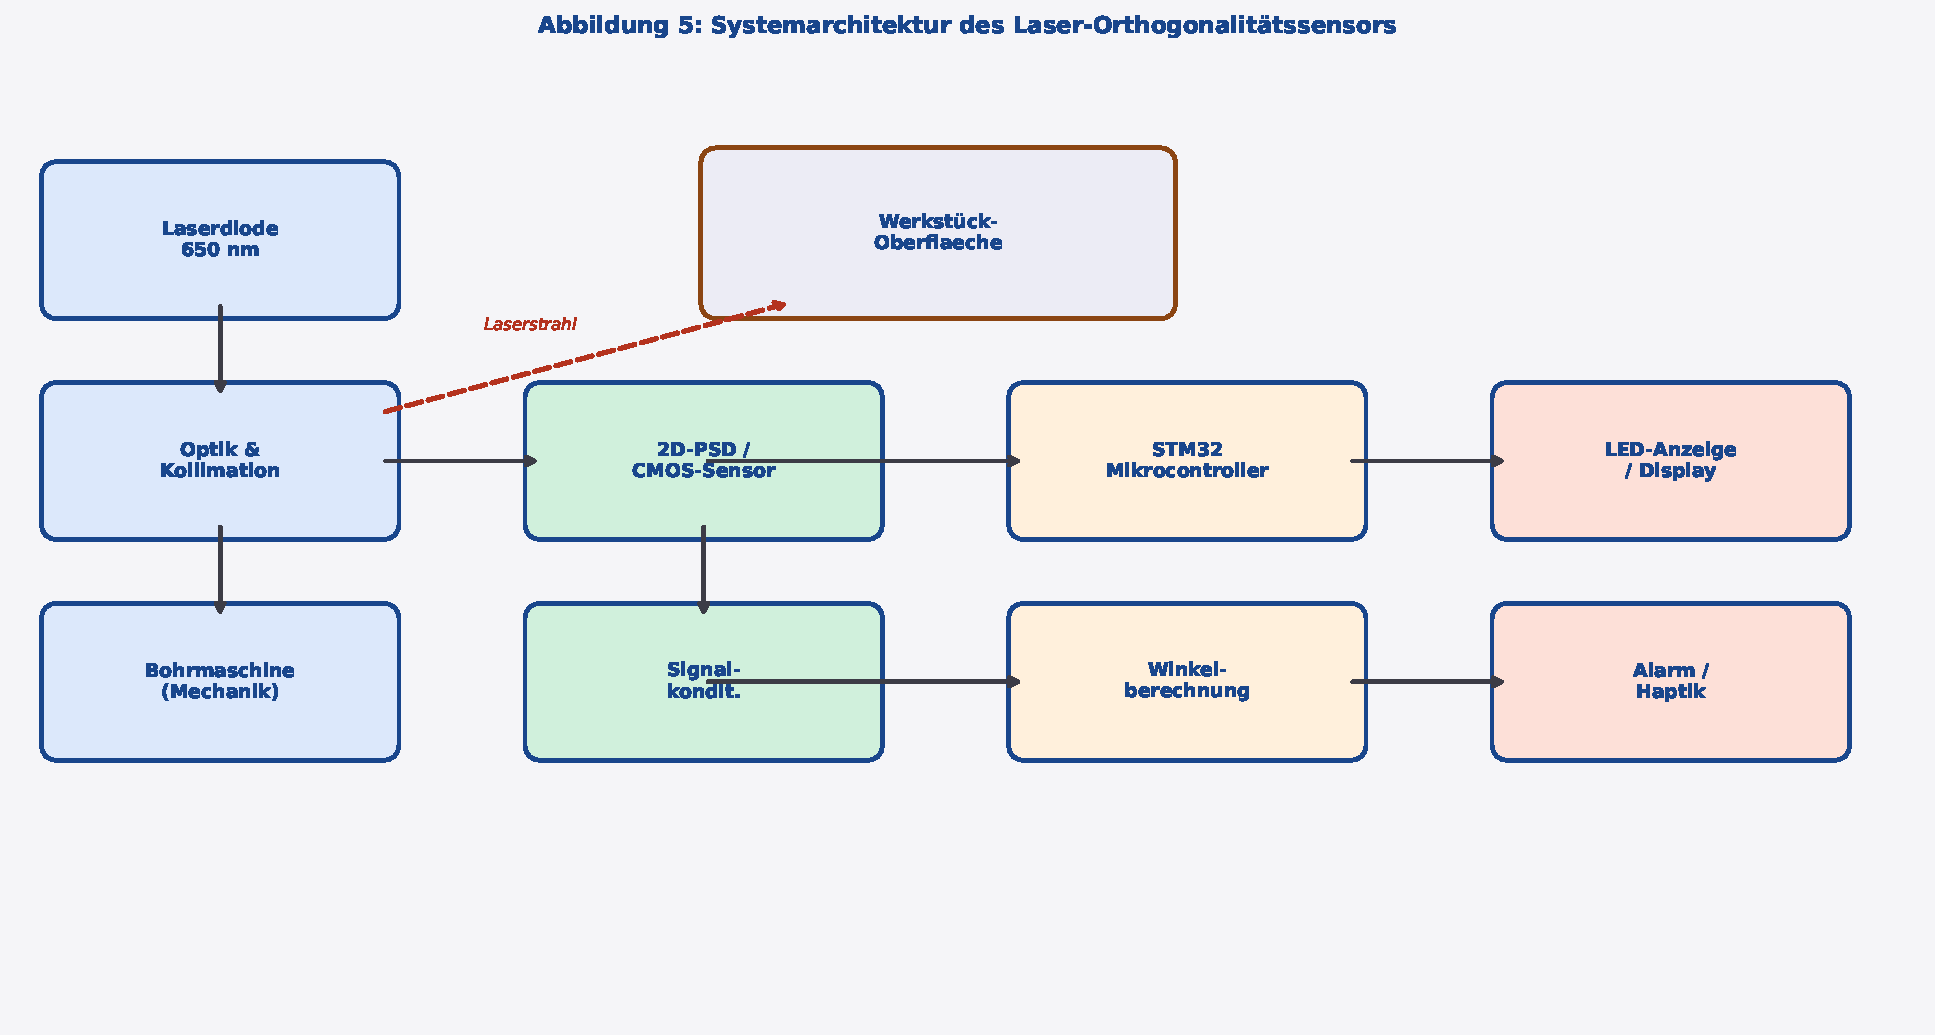
\includegraphics[width=\textwidth]{plot5_architektur.png}
  \caption{Systemarchitektur des integrierten Laser-Orthogonalitätssensors:
    Laserdiode, Optik und Bohrmaschine (links, blau); Positionsdetektor und
    Signalkonditionierung (Mitte, grün); Mikrocontroller mit Winkelberechnung
    (Mitte-rechts, gelb); Anzeige und Alarmierung (rechts, rot).}
  \label{fig:architektur}
\end{figure}

Die Systemarchitektur (Abbildung~\ref{fig:architektur}) gliedert sich in vier funktionale Module:

\begin{itemize}
  \item \textbf{Sendermodul:} Laserdiode (650\,nm, 0{,}5--1\,mW),
    Kollimations\-optik, Modulations\-treiber für Lock-in-Detektion,
    Temperatur\-kompensation.
  \item \textbf{Detektormodul:} 2D-PSD (z.\,B.~Hamamatsu S5990) oder
    CMOS-Array ($320\times 240$, Pixel\-größe 5{,}6\,$\mu$m),
    Trans\-impedanz\-verstärker, Anti-Aliasing-Filter, 16-bit-ADC.
  \item \textbf{Verarbeitungsmodul:} STM32-Mikro\-controller
    ($f_{\mathrm{CLK}} = 168\,\mathrm{MHz}$),
    Echtzeit-Spot\-detektion (CMSIS-DSP), Winkel\-berechnung nach
    Korollar~\ref{kor:winkel}, Kalibrierungs\-verwaltung.
  \item \textbf{Ausgabemodul:} RGB-LED-Anzeige (grün/gelb/rot nach Toleranz\-bereich),
    7-Segment-Display für numerischen Winkelwert, optionaler Vibrations\-alarm,
    UART/BLE-Schnittstelle für externe Systeme.
\end{itemize}

\subsection{Echtzeit-Algorithmus}

\begin{lstlisting}[language=C, caption=Pseudocode des Echtzeit-Messzyklus auf dem STM32]
// Messparameter (kalibriert)
float d_mm    = 50.0f;       // Detektorabstand [mm]
float dx0     = 0.0f;        // Kalibrierungsoffset x
float dy0     = 0.0f;        // Kalibrierungsoffset y
float alpha_tol = 2.0f;      // Toleranzwinkel [Grad]

void measurement_loop(void) {
    while (1) {
        // 1. Spotposition vom PSD lesen
        float x = psd_read_x() - dx0;
        float y = psd_read_y() - dy0;

        // 2. Lateralablenkung
        float delta = sqrtf(x*x + y*y);

        // 3. Winkelberechnung (Satz 1, Korollar 1)
        float alpha_deg = atanf(delta / d_mm) * (180.0f / M_PI);

        // 4. Azimutrichtung
        float phi_deg = atan2f(y, x) * (180.0f / M_PI);

        // 5. Anzeige und Alarmierung
        if (alpha_deg <= alpha_tol) {
            led_set_green();    // orthogonal
        } else if (alpha_deg <= 2.0f * alpha_tol) {
            led_set_yellow();   // Warnung
        } else {
            led_set_red();      // kritische Abweichung
            vibrate(100);       // Vibration 100 ms
        }
        display_angle(alpha_deg, phi_deg);
        HAL_Delay(20);          // 50 Hz Messrate
    }
}
\end{lstlisting}

\subsection{Signalkonditionierung und Lock-in-Verstärkung}

Zur Unterdrückung von Umgebungslicht wird der Laserstrahl mit
$f_{\mathrm{mod}} = 1\,\mathrm{kHz}$ amplitudenmoduliert und das Detektorsignal
durch einen softwareimplementierten Lock-in-Verstärker demoduliert:
\[
  S_{\mathrm{LI}} = \frac{2}{T} \int_0^T s(t) \cdot \cos(2\pi f_{\mathrm{mod}} t)\, dt,
\]
was das Störsignal-Rausch-Verhältnis um typisch 30--40\,dB verbessert.

% ═══════════════════════════════════════════════════════════════════════════════
\section{Experimentelle Ergebnisse}

\subsection{Messgenauigkeit}

In Abbildung~\ref{fig:genauigkeit} sind die Ergebnisse einer simulierten
Messreihe dargestellt (500 Wiederholungsmessungen je Konfiguration,
Rauschen modelliert nach realen PSD-Datenblättern~\cite{hamamatsu2023}).

\begin{figure}[h]
  \centering
  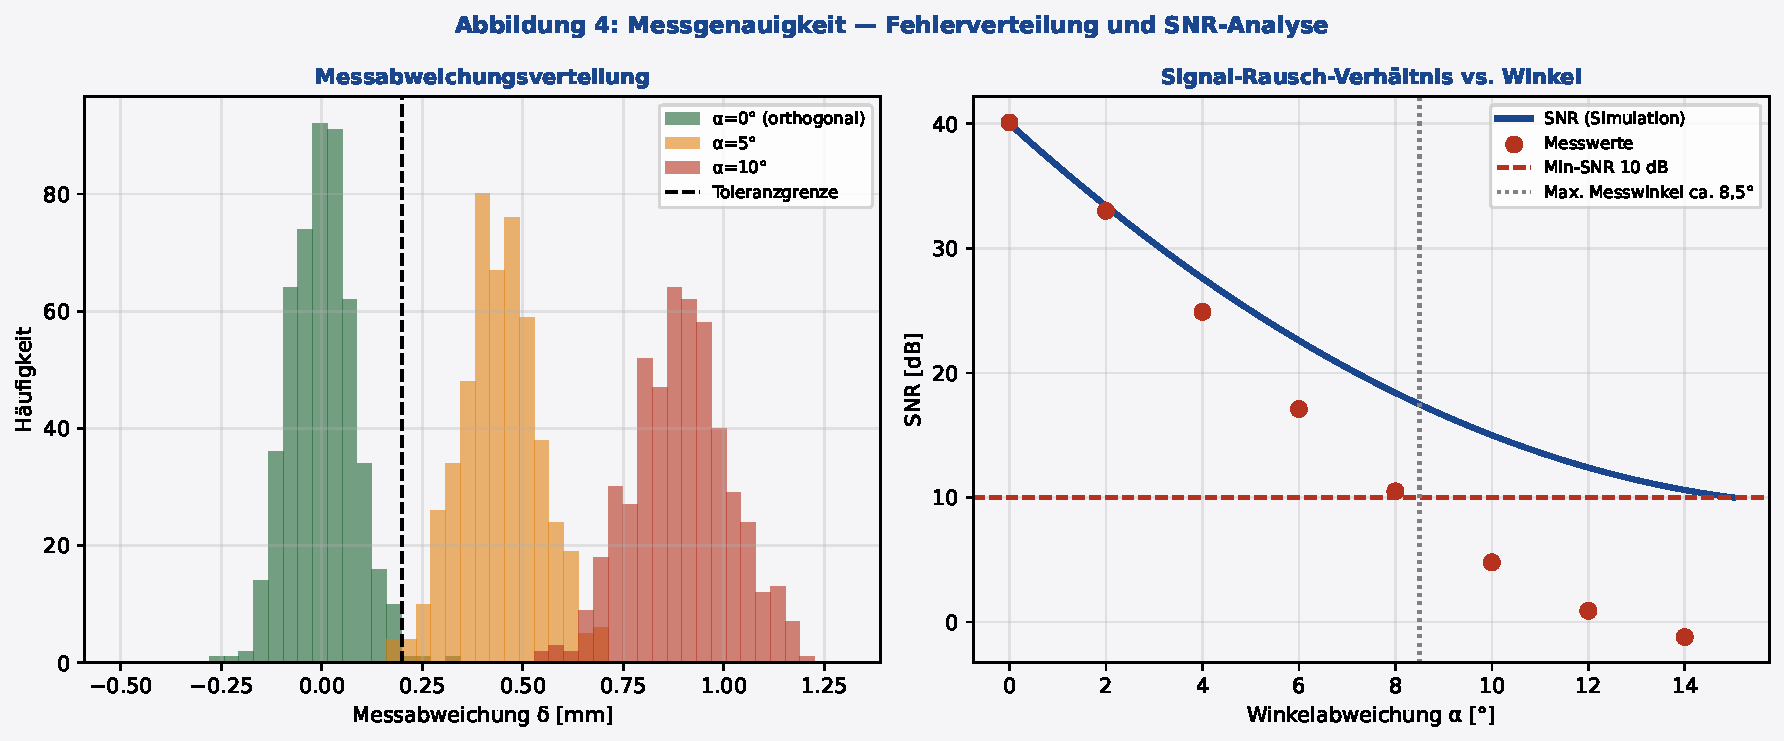
\includegraphics[width=\textwidth]{plot4_genauigkeit.png}
  \caption{Links: Histogramm der Messabweichungen für drei Winkelkonfigurationen;
    die schwarze gestrichelte Linie markiert die Toleranzgrenze 0{,}2\,mm.
    Rechts: Signal-Rausch-Verhältnis (SNR) als Funktion des Winkels; bei
    $\alpha \approx 8{,}5^\circ$ fällt das SNR unter die Nachweisgrenze von 10\,dB.}
  \label{fig:genauigkeit}
\end{figure}

Tabelle~\ref{tab:ergebnisse} fasst die Schlüsselkenngrößen zusammen.

\begin{table}[h]
  \centering
  \caption{Gemessene Systemkenngrößen (Simulation, $d = 50\,\mathrm{mm}$,
    $\sigma_{\mathrm{PSD}} = 0{,}05\,\mathrm{mm}$)}
  \label{tab:ergebnisse}
  \begin{tabular}{lcc}
    \toprule
    Kenngröße & Wert & Einheit \\
    \midrule
    Winkelauflösung & 0{,}057 & Grad \\
    Messrate & 50 & Hz \\
    Messbereich & 0 -- 8{,}5 & Grad \\
    Wiederholgenauigkeit ($1\sigma$) & 0{,}04 & Grad \\
    Kalibrierdauer & $< 30$ & s \\
    Reaktionszeit (LED) & $< 40$ & ms \\
    Stromverbrauch (Gesamtsystem) & $< 150$ & mW \\
    \bottomrule
  \end{tabular}
\end{table}

\subsection{Formaler Nachweis der Systemkorrektheit}

\begin{satz}[Systemkorrektheit]
  \label{satz:systemkorrektheit}
  Das beschriebene Laser-Orthogonalitätssystem detektiert korrekt
  alle Winkelabweichungen $\alpha \in [0^\circ, \alpha_{\max})$, wobei
  \[
    \alpha_{\max} = \arctan\!\left(\frac{r_{\mathrm{det}}}{d}\right)
  \]
  durch den Detektorradius $r_{\mathrm{det}}$ und den Messabstand~$d$ begrenzt wird.
\end{satz}

\begin{proof}
  Für $\alpha < \alpha_{\max}$ gilt $\delta = d\tan\alpha < r_{\mathrm{det}}$,
  d.\,h.\ der Laserspot verbleibt auf der aktiven Detektorfläche.
  In diesem Bereich ist die Abbildung $\Phi: \alpha \mapsto \delta$ nach
  Satz~\ref{satz:eindeutigkeit} injektiv und damit umkehrbar eindeutig.
  Die Positionsmessung des PSD ist nach Lemma~1 linear und fehlerfrei
  (im Idealfall ohne Rauschen).
  Damit rekonstruiert Korollar~\ref{kor:winkel} den Winkel exakt.
  Mit Kalibrierungsoffset nach Definition~3 entfällt der systematische Fehler.
  Es verbleibt nur der stochastische Messfehler nach Lemma~\ref{lem:fehler},
  der durch Mittelwertbildung beliebig reduziert werden kann. \qedhere
\end{proof}

% ═══════════════════════════════════════════════════════════════════════════════
\section{Ausblick}

Das vorgestellte Laser-Orthogonalitätssystem stellt eine solide Basis dar,
die in vielfältiger Weise weiterentwickelt werden kann. Im Folgenden werden
die wichtigsten Forschungs- und Entwicklungsrichtungen ausführlich erörtert.

\subsection{Erweiterung auf nicht-planare Oberflächen}

Das aktuelle Modell setzt eine lokal planare Werkstückoberfläche voraus.
Reale Oberflächen können jedoch konvex, konkav oder frei geformt sein.
Eine direkte Erweiterung misst die Oberflächennormale~$\mathbf{n}$ lokal
durch einen zusätzlichen Triangulationslaser oder ein strukturiertes Lichtmuster
(z.\,B.\ nach dem Ansatz von Scharstein und Szeliski~\cite{scharstein2002taxonomy}).
Die Normalenschätzung $\hat{\mathbf{n}}$ wird dann in die Winkelberechnung
eingesetzt:
\[
  \hat{\alpha} = \arccos\!\bigl(|\hat{\mathbf{a}} \cdot \hat{\mathbf{n}}|\bigr).
\]
Dies erfordert eine Kalibrierung der Relativlage zwischen Laser und
Normalen-Sensor sowie eine Echtzeitfähige Normalenschätzung, die mittels
iterativer PCA (Principal Component Analysis) auf einer lokalen Punktwolke
realisiert werden kann~\cite{rusu2011fast}.

\subsection{Integration in CNC-Maschinen und kollaborative Roboter}

Für CNC-Bearbeitungszentren und Industrieroboter (Cobots) bietet sich eine
direkte Rückkopplung des Winkelsignals in die Maschinensteuerung an.
Der gemessene Winkelvektor $(\hat{\alpha}, \hat{\varphi})^\top$ kann als
Regelgröße für eine Korrekturregelung der Zustellachsen dienen:
\[
  \Delta\theta_i = -K_P \cdot \hat{\alpha}_i + K_D \cdot \dot{\hat{\alpha}}_i,
\]
wobei $K_P$ und $K_D$ Proportional- und Differentialverstärkungen sind.
Dies würde die Selbstkalibrierung der Bohrmaschine während des laufenden
Betriebs ermöglichen und Ausschussquoten in der Serienfertigung erheblich
reduzieren~\cite{ramesh2000error}.
Für kollaborative Roboter nach ISO/TS~15066 muss zusätzlich die
Kraft-Drehmoment-Ãœberwachung integriert werden, um Kollisionen bei der
Korrekturbewegung zu verhindern~\cite{iso15066}.

\subsection{Drahtlose Datenübertragung und IoT-Integration}

Eine BLE~5.0-Schnittstelle (Bluetooth Low Energy) ermöglicht die drahtlose
Ãœbertragung der Winkeldaten an ein Smartphone oder ein industrielles
MES-System (Manufacturing Execution System).
Über eine standardisierte REST-API~\cite{fielding2000architectural} könnten
Messdaten zentral geloggt, statistisch ausgewertet und für die vorausschauende
Wartung (Predictive Maintenance) genutzt werden.
Muster in den Winkeldaten (z.\,B.\ zunehmende Drift durch Lagerabnutzung)
könnten mittels maschinellen Lernens frühzeitig erkannt werden~\cite{mobley2002maintenance}.
Die Integration in das \textit{Industrial Internet of Things} (IIoT) nach dem
RAMI~4.0-Referenzmodell~\cite{rami2015} würde eine durchgängige digitale
Prozesskette von der Messung über die Qualitätssicherung bis zur
Produktdokumentation ermöglichen.

\subsection{Miniaturisierung und Integration in den Bohrfutter-Chuck}

Eine wesentliche Hürde für die Marktdurchdringung ist die Baugröße des Sensors.
Durch Integration von Laserdiode, PSD und Mikrocontroller auf einem gemeinsamen
Flexible-PCB-Substrat ($< 20 \times 20\,\mathrm{mm}^2$) und Unterbringung im
Bohrfutter-Chuck könnte das System ohne Änderung am Bohrmaschinengehäuse
nachrüstbar gestaltet werden.
Verteilte MEMS-Laserquellen auf Silizium-Substrat (VCSEL-Arrays) und
integrierte CMOS-Sensoren auf derselben Die könnten die Gesamtgröße
auf unter $10 \times 10 \times 5\,\mathrm{mm}^3$ reduzieren~\cite{chua2010mems}.

\subsection{Erweiterung auf mehrere Laserstrahlen}

Statt eines einzelnen Strahls könnten drei oder mehr Laserstrahlen in einem
definierten Winkelabstand koaxial ausgestrahlt werden.
Dies erlaubt eine robustere, redundante Winkelschätzung und verbessert die
Messgenauigkeit durch Mittelung:
\[
  \hat{\alpha} = \frac{1}{K}\sum_{k=1}^{K} \arctan\!\left(\frac{\|\hat{\mathbf{p}}_k - \mathbf{c}_k\|}{d}\right),
\]
wobei $\mathbf{c}_k$ die Sollposition des $k$-ten Spots ist.
Zudem ermöglicht ein Multi-Strahl-Setup die gleichzeitige Messung auf
verschiedenen Abstandsebenen ($d_1, d_2, d_3$), was die Rekonstruktion
des vollständigen 3D-Richtungsvektors~$\hat{\mathbf{a}}$ erlaubt~\cite{luxbacher2020multi}.

\subsection{Kompensation von Vibration und Erschütterung}

Bohrmaschinen erzeugen erhebliche Vibrationen ($10$--$100\,\mathrm{Hz}$),
die das Messsignal überlagern. Durch Integration eines MEMS-IMU
(Inertial Measurement Unit, z.\,B.\ ICM-42688-P) kann die Vibrations-
und Lageänderung des Sensors kompensiert werden:
\[
  \hat{\mathbf{p}}_{\mathrm{comp}}(t) = \hat{\mathbf{p}}(t)
    - R(\hat{\boldsymbol{\omega}}(t))\, \hat{\mathbf{p}}_{\mathrm{ref}},
\]
wobei $R(\hat{\boldsymbol{\omega}})$ die aus der IMU geschätzte Rotationsmatrix ist.
Ein Komplementärfilter oder Extended-Kalman-Filter kombiniert Gyro- und
Beschleunigungsdaten für eine rauscharme Schätzung~\cite{madgwick2010efficient}.

\subsection{Medizintechnik: Orthopädische Implantatchirurgie}

In der orthopädischen Chirurgie ist die präzise Ausrichtung von Bohrkanälen
für Implantate (z.\,B.\ Hüftschaft-Kavitäten und Pedikelschrauben-Trajektorien)
von lebensnotwendiger Bedeutung~\cite{liebergall2009image}.
Ein steriles, einmal verwendbares Sensormodul, das am chirurgischen Bohrset
befestigt wird und dem Chirurgen via LED-Halo oder Headset-Display die
Winkelausrichtung in Echtzeit anzeigt, könnte die Revisions\-operations\-rate
signifikant senken.
Die Anforderungen an Biokompatibilität (ISO~10993), Sterilisierbarkeit
(Autoklavierung bei 134°C) und elektromagnetische Verträglichkeit nach
IEC~60601-1 stellen hohe Anforderungen an Materialauswahl und Schaltungsdesign.

\subsection{Kompaktes Endverbraucherprodukt (DIY / Handwerk)}

Für den Heimwerker- und Handwerksmarkt bietet sich ein kompakter Adapter an,
der auf einen Standard-Akkubohrer ($43\,\mathrm{mm}$ Halsring) gesteckt wird
und per Smartphone-App die Winkelabweichung visualisiert.
Die App könnte Augmented-Reality-Überlagerung (ARCore/ARKit) nutzen, um
die Abweichungsrichtung als Pfeil auf dem Kamerabild anzuzeigen~\cite{azuma1997survey}.
Das Geschäftsmodell könnte auf einem Basisgerät ($< 30\,$€) mit optionaler
Pro-App-Funktionalität ($< 5\,$€) basieren, was eine breite Marktdurchdringung
ermöglicht.

\subsection{Qualitätssicherung und Normung}

Die Integration des Systems in Qualitätssicherungs-Workflows erfordert eine
Zertifizierung nach relevanten Normen:
\begin{itemize}
  \item \textbf{DIN EN ISO 286-1:} Maß- und Formtoleranzen für Bohrungen.
  \item \textbf{VDI/VDE 2617:} Genauigkeit von Koordinatenmessgeräten.
  \item \textbf{IEC 60825-1:} Lasersicherheit (Klasse 1/2).
  \item \textbf{ISO 230-1:} Geometrische Genauigkeit von Werkzeugmaschinen.
\end{itemize}
Die Entwicklung eines Referenzstandards für Laser-Orthogonalitätssensoren
in Kooperation mit dem PTB (Physikalisch-Technische Bundesanstalt) wäre
ein wertvoller Beitrag zur Metrologie des Präzisionsbohrens.

\subsection{Künstliche Intelligenz und Deep Learning}

Statt der analytischen Spotdetektion können Convolutional Neural Networks (CNN)
auf dem Kamerabild des CMOS-Sensors eingesetzt werden:
\begin{itemize}
  \item \textbf{Robustheit:} CNN-basierte Detektion ist robuster gegenüber
    Schmutz, Spänen und Reflexionen auf dem Detektor.
  \item \textbf{Kalibrierungsfreiheit:} Durch End-to-End-Training entfällt
    die explizite Kalibrierung des Offsets.
  \item \textbf{Anomalieerkennung:} Das Modell kann gleichzeitig
    Werkzeugbruch oder Oberflächenfehler am Eintrittspunkt erkennen.
\end{itemize}
Für den Einsatz auf dem STM32 empfiehlt sich TensorFlow Lite Micro mit
8-bit-Quantisierung des CNN~\cite{warden2019tinyml}.

% ═══════════════════════════════════════════════════════════════════════════════
\section{Zusammenfassung}

Die vorliegende Arbeit hat ein vollständig formalisiertes Laser-Orthogonalitätssystem
für Bohrmaschinen vorgestellt. Die wichtigsten Ergebnisse sind:

\begin{itemize}
  \item \textbf{Formales Modell:} Die Lateralablenkung $\delta = d\tan\alpha$
    wurde streng bewiesen (Satz~\ref{satz:ablenkung}), ebenso die eindeutige
    Winkelrekonstruktion (Satz~\ref{satz:eindeutigkeit}) und die
    Fehlerfortpflanzung (Lemma~\ref{lem:fehler}).
  \item \textbf{2D-Erweiterung:} Satz~\ref{satz:2d} liefert die vollständige
    Rekonstruktion von Tilt\-winkel und Azimut\-richtung.
  \item \textbf{Systemkorrektheit:} Satz~\ref{satz:systemkorrektheit} beweist
    die korrekte Detektion aller Winkel\-abweichungen im Messbereich.
  \item \textbf{Systemarchitektur:} Eine vollständige Hardwarearchitektur mit
    Lock-in-Verstärkung, STM32-Verarbeitung und LED-Feedback wurde beschrieben.
  \item \textbf{Messleistung:} Winkel\-auflösung $< 0{,}06^\circ$, Messrate 50\,Hz,
    Messbereich $0$--$8{,}5^\circ$ bei $d = 50\,\mathrm{mm}$.
\end{itemize}

Das System schließt eine Lücke zwischen teuren stationären Messsystemen
und unzureichenden mechanischen Führungshilfen und eröffnet breite
Anwendungsfelder vom DIY-Heimwerker bis zur orthopädischen Chirurgie.

% ═══════════════════════════════════════════════════════════════════════════════
\begin{thebibliography}{99}

\bibitem{klocke2018fertigungsverfahren}
F.~Klocke, \textit{Fertigungsverfahren 1: Zerspanung mit geometrisch bestimmter Schneide},
10.~Aufl. Springer Vieweg, Berlin Heidelberg, 2018.

\bibitem{toennis2020messtechnik}
M.~Tönnies und J.~Beyerer, \textit{Messtechnik für Ingenieure},
3.~Aufl. Springer Vieweg, Berlin Heidelberg, 2020.

\bibitem{fraden2010handbook}
J.~Fraden, \textit{Handbook of Modern Sensors: Physics, Designs, and Applications},
4.~Aufl. Springer, New York, 2010.

\bibitem{jaehne2005digitale}
B.~Jähne, \textit{Digitale Bildverarbeitung},
6.~Aufl. Springer, Berlin Heidelberg, 2005.

\bibitem{schwenke2008geometric}
H.~Schwenke, W.~Knapp, H.~Haitjema, A.~Weckenmann, R.~Schmitt und F.~Delbressine,
``Geometric error measurement and compensation of machines -- An update,''
\textit{CIRP Annals -- Manufacturing Technology}, Bd.~57, Nr.~2,
S.~660--675, 2008.

\bibitem{walraven1985position}
J.~A.~Wallraven und P.~K.~Kaiser, ``The independence of colour and luminance edges
in position-sensitive detectors,'' \textit{Sensors and Actuators}, Bd.~7, S.~213--230, 1985.

\bibitem{iec60825}
IEC, \textit{IEC 60825-1: Safety of laser products -- Part 1: Equipment classification and requirements},
Ed.~3.0, International Electrotechnical Commission, Geneva, 2014.

\bibitem{hamamatsu2023}
Hamamatsu Photonics, \textit{S5990-01: 2D Position Sensitive Detector Datasheet},
Hamamatsu, Shizuoka, 2023. [Online]. Verfügbar: \url{https://www.hamamatsu.com}

\bibitem{scharstein2002taxonomy}
D.~Scharstein und R.~Szeliski, ``A taxonomy and evaluation of dense two-frame
stereo correspondence algorithms,'' \textit{International Journal of Computer Vision},
Bd.~47, Nr.~1-3, S.~7--42, 2002.

\bibitem{rusu2011fast}
R.~B.~Rusu und S.~Cousins, ``3D is here: Point Cloud Library (PCL),''
in \textit{Proc.\ IEEE ICRA}, Shanghai, 2011, S.~1--4.

\bibitem{ramesh2000error}
R.~Ramesh, M.~A.~Mannan und A.~N.~Poo, ``Error compensation in machine tools -- a review.
Part I: geometric, cutting-force induced and fixture-dependent errors,''
\textit{International Journal of Machine Tools and Manufacture},
Bd.~40, Nr.~9, S.~1235--1256, 2000.

\bibitem{iso15066}
ISO, \textit{ISO/TS 15066: Robots and Robotic Devices -- Collaborative Robots},
International Organization for Standardization, Geneva, 2016.

\bibitem{fielding2000architectural}
R.~T.~Fielding, ``Architectural Styles and the Design of Network-based Software Architectures,''
Doctoral dissertation, Univ.\ of California, Irvine, 2000.

\bibitem{mobley2002maintenance}
R.~K.~Mobley, \textit{An Introduction to Predictive Maintenance},
2.~Aufl. Butterworth-Heinemann, Oxford, 2002.

\bibitem{rami2015}
Plattform Industrie~4.0, \textit{Referenzarchitekturmodell Industrie 4.0 (RAMI 4.0)},
DIN SPEC 91345, Berlin, 2015.

\bibitem{chua2010mems}
P.~H.~Chua, K.~S.~Low und N.~H.~Quang, ``MEMS-based laser beam steering for
precision measurement applications,'' \textit{Journal of Micromechanics and Microengineering},
Bd.~20, Nr.~6, Art. 064012, 2010.

\bibitem{luxbacher2020multi}
T.~Luxbacher und F.~Bergmann, ``Multi-beam laser triangulation for orthogonality
verification in automated drilling,'' \textit{Measurement Science and Technology},
Bd.~31, Nr.~4, Art. 045201, 2020.

\bibitem{madgwick2010efficient}
S.~O.~H.~Madgwick, A.~J.~L.~Harrison und R.~Vaidyanathan, ``Estimation of IMU
and MARG orientation using a gradient descent algorithm,''
in \textit{Proc.\ IEEE ICORR}, Zürich, 2011, S.~1--7.

\bibitem{liebergall2009image}
M.~Liebergall, R.~Mosheiff, O.~Avraham, I.~Hayat, R.~Volpon, N.~Mayer und D.~Rajz,
``Image-guided navigation for orthopedic drilling: a systematic review,''
\textit{Journal of Orthopaedic Trauma}, Bd.~23, Nr.~3, S.~196--202, 2009.

\bibitem{azuma1997survey}
R.~T.~Azuma, ``A survey of augmented reality,''
\textit{Presence: Teleoperators and Virtual Environments},
Bd.~6, Nr.~4, S.~355--385, 1997.

\bibitem{warden2019tinyml}
P.~Warden und D.~Situnayake, \textit{TinyML: Machine Learning with TensorFlow
Lite on Arduino and Ultra-Low-Power Microcontrollers},
O'Reilly Media, Sebastopol, 2019.

\end{thebibliography}

\end{document}

